\documentclass[en]{../../../../../../eplexam}

\usepackage{../../../../../../eplunits}

\graphicspath{{img/}}

\hypertitle{Radiation and communication systems}{7}{ELEC}{2795}{2020}{Janvier}{All}
{Martin Braquet \and Sébastien Couvreur \and Oriane de Leuze}
{Christophe Craeye, Danielle Janvier, Jérome Louveaux, Claude Oestges and Luc Vandendorpe}

\section{(4,5 points)}
A ground station is emitting a plane wave toward a satellite, with an elevation angle $\alpha_1=10^o$. The electric field is horizontally polarized. The atmosphere is modelled as two dielectric layers separated by a horizontal interface. The relative dielectric permittivity of the two layers is $\epsilon_1$ and $\epsilon_2 = 1.01\epsilon_1$ respectively.

\begin{figure}[!h]
    \centering
    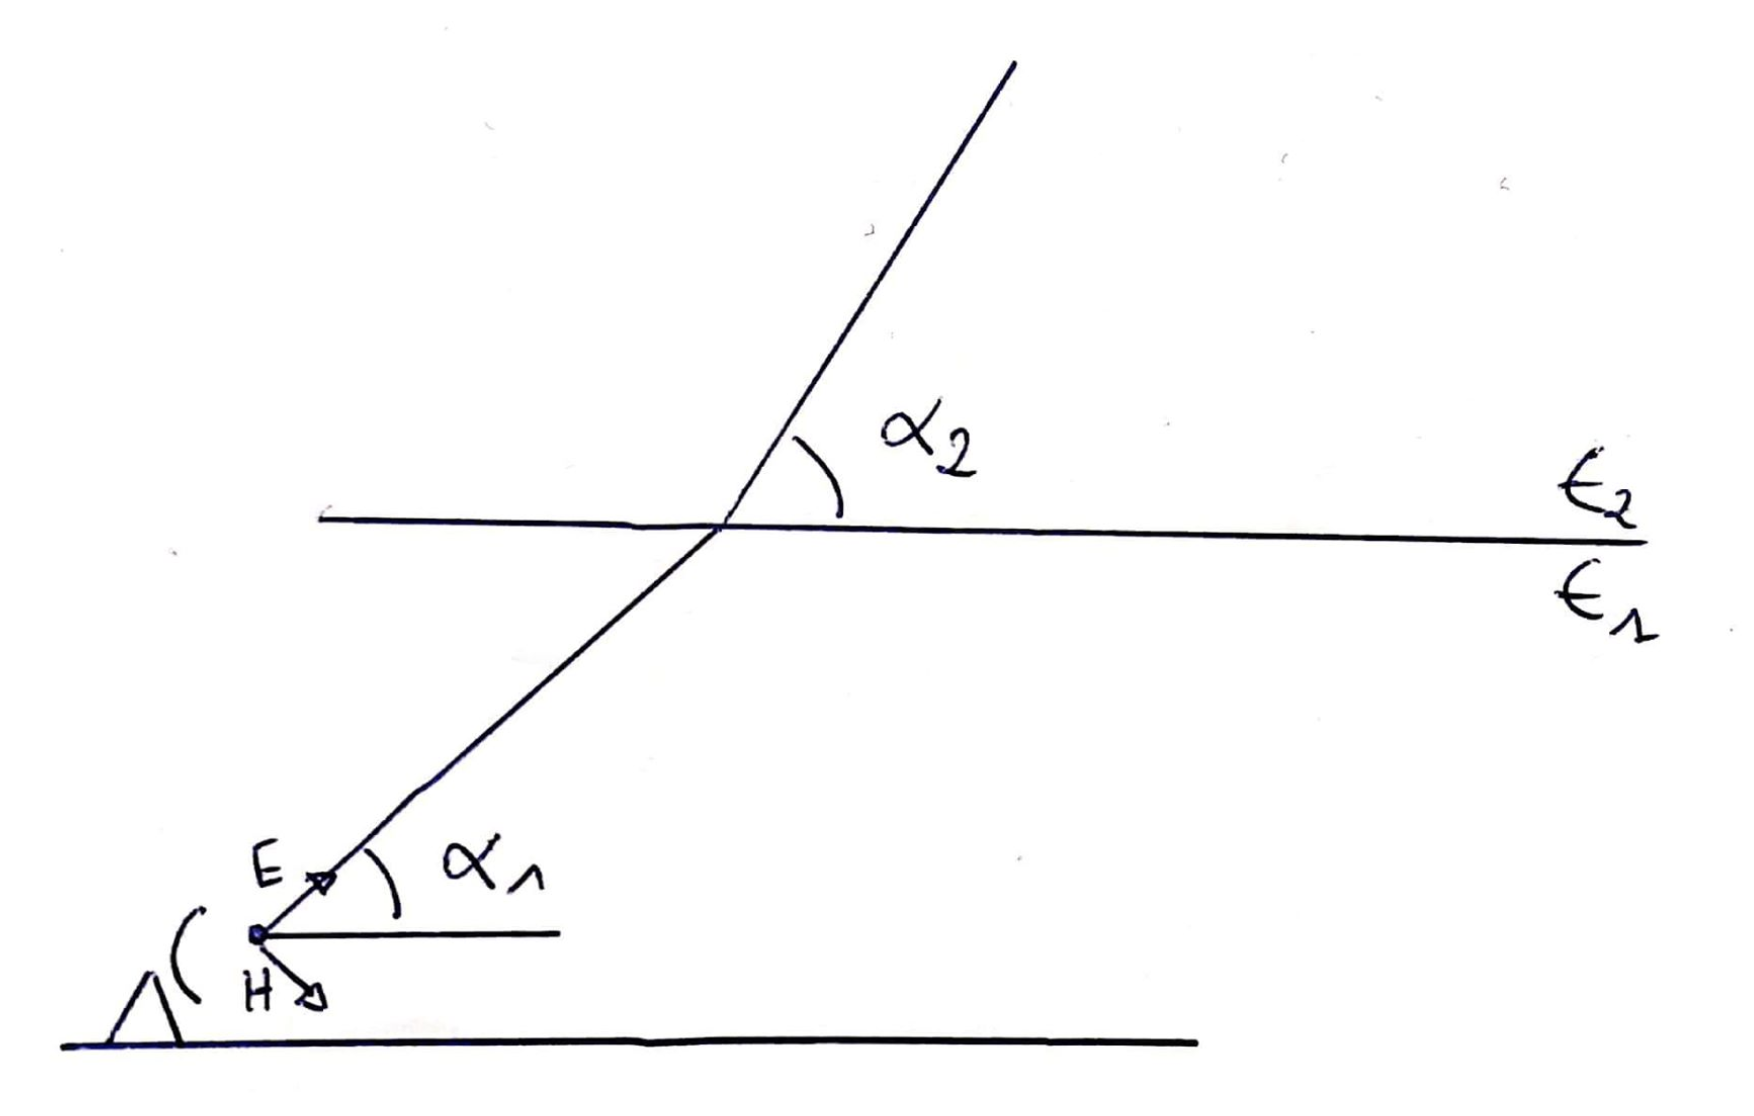
\includegraphics[scale=0.3]{Q1.png}
\end{figure}

\begin{enumerate}
    \item (1 point) Calculate the elevation angle in layer 2 ($\alpha_2$ in the figure).
    \item (2 point) Calculate the reflection coefficient $\Gamma$ and the transmission coefficient $T$ of the electric field at the interface between the two layers.
    \item (1,5 points) If the distance between the satellite and the ground station (Matera) is \SI{40500}{km} and the frequency \SI{7.8}{GHz}, calculate the free space losses + total tropospheric losses exceeded during 0.01\% of the time.
\end{enumerate}
(CCDF graph available with an attenuation of \SI{9}{dB} for 0.01\% of the time at the angle and frequency related to this problem)

\nosolution


\section{(4,5 points)}

Two parabolic dish antennas are facing each other to establish a horizontal link over a distance of \SI{2}{km}. The frequency of operation is \SI{5}{GHz} and the diameter of the dishes is 1 meter. Both antennas have an input impedance of \SI{50}{\ohm}, while the generator impedance is $(100-j50)$ Ohm on the transmitting side and the receiver impedance is \SI{50}{\ohm} on the receiving side. The noise figure of the receiver is \SI{3}{dB}, the bandwidth of the signal is \SI{5}{MHz}. The transmitting polarization is vertical, while the receiving polarization is circular. \SI{10}{mW} are available at the generator.
\begin{enumerate}
    \item Assuming in a first instance that the two antennas have the same polarization and that they are impedance matched, what is the signal-to-noise ratio on the receiver?
    \item What does that SNR become with the impedance and polarization mismatches referred to above?
    \item With which accuracy (in degrees) do the two antennas need to be pointed at each other to avoid a decrease of the signal by more than \SI{3}{dB}? (do the calculation assuming that one antenna is perfectly pointed and the other is not)
\end{enumerate}

\nosolution


\section{(4,5 points)}

We consider the downlink of a cellular transmission \SI{3.5}{GHz}, using a bandwidth of \SI{5}{MHz} per user. At the base station, the transmit power is 20 W and the antenna gain is \SI{5}{dBi}. For the considered environment, the path-loss is given in [\si{dB}] by:
\[ P_L [\si{dB}] = 140 + 10 \gamma \log_{10}(d) + S_{\si{dB}} \]
where $d$ is the distance in km from the base station , $\gamma = 3$ is the pass-loss exponent and $S_\si{dB}$ is the log-normal shadowing: $S_\si{dB}$ is a zero-mean Gaussian variable with a standard deviation of \SI{6}{dB}.
The mobile terminal is characterized by a quasi-omnidirectional antenna of \SI{2}{dBi} gain and a noise spectral density of \SI{1.9e-19}{mW/Hz}.
\begin{enumerate}
    \item What should be the cell radius $R$ in order to guarantee that the average received power is at least \SI{-100}{dBm} over the entire cell?
    \item What is therefore the average SNR (received power to noise power ratio) at the cell edge (i.e. at a distance $d=R$)?
    \item What is the probability that the received power falls bellow \SI{-114}{dBm} at the cell edge?
    \item Assuming hexagonal cells, at which distance can the network operator re-use the same frequency to maintain a Signal-to-Interference Ratio (SIR) of \SI{18}{dB} (neglecting thermal noise)? What is in this case the cell pattern (i.e. the number of available frequencies)?
    \item If the channel consists in two multi-paths of equal amplitude, what is the maximum separation in delay that could still guarantee flat-fading transmission? Is this realistic in urban areas?
\end{enumerate}
Appendix - Cumulative distribution of standard normal variable (zero-mean Gaussian with unit variance)\\
(Probability table available)


\nosolution

\section{(4,5 points)(+0.5 if correct, 0 otherwise)}

\begin{enumerate}
    \item \textbf{Which one of the following is true regarding the difference between DMT and OFDM?}
    \begin{enumerate}
        \item OFDM could be used instead of DMT in a DSL system but its bitrate would be reduced
        \item DMT could be used instead of OFDM in a wireless system before modulation at the carrier frequency but its bitrate would be reduced
        \item OFDM and DMT are completely different and can never be interchanged
        \item OFDM and DMT are completely equivalent and can always be interchanged
    \end{enumerate}
    \item \textbf{The RFI usually impacts}
    \begin{enumerate}
        \item The whole bandwidth of DSL systems
        \item A few very small bands
        \item One large part of the band
        \item Only ADSL and VDSL but not later generations
    \end{enumerate}
    \item \textbf{TDD is chosen as the duplexing method instead of FDD in G.Fast because}
    \begin{enumerate}
        \item NEXT is no longer present in G.Fast
        \item The upstream has a much lower bitrate in G.Fast
        \item In earlier versions, it was difficult to synchronize all the lines but TDD allows more flexibility
        \item It was impossible to create bandplans that are compatible with VDSL
    \end{enumerate}
    \item \textbf{The DSL profile (bandplan) 12a uses 2783 tones (with usual spacing). Which standard is it coming from?}
    \begin{enumerate}
        \item ADSL
        \item ADSL2+
        \item VDSL2
        \item G.Fast
    \end{enumerate}
    \item
    \item \textbf{Over channels experiencing fading, when the number of diversity elements/sources is increased, in the best case}
    \begin{enumerate}
        \item The SNR becomes the one achieved over an AWGN channel
        \item The SNR can be higher than over an AWGN channel
    \end{enumerate}
    \item 
    \item
    \item \textbf{For a fixed carrier frequency, increasing the number of subcarriers in OFDM will}
    \begin{enumerate}
        \item Improve the data transmission
        \item Worsen the data transmission
        \item Not change the data transmission
    \end{enumerate}
\end{enumerate}

\nosolution

\end{document}
